%%%%%%%%%%%%%%%%%%%%%%%%%%%%%%%%%%%%%%%%%%%%%%%%%%%%%%%%%%%%%%%
%% OXFORD THESIS TEMPLATE

% Use this template to produce a standard thesis that meets the Oxford University requirements for DPhil submission
%
% Originally by Keith A. Gillow (gillow@maths.ox.ac.uk), 1997
% Modified by Sam Evans (sam@samuelevansresearch.org), 2007
% Modified by John McManigle (john@oxfordechoes.com), 2015
%
% This version Copyright (c) 2015-2017 John McManigle
%
% Broad permissions are granted to use, modify, and distribute this software
% as specified in the MIT License included in this distribution's LICENSE file.
%

% I've (John) tried to comment this file extensively, so read through it to see how to use the various options.  Remember
% that in LaTeX, any line starting with a % is NOT executed.  Several places below, you have a choice of which line to use
% out of multiple options (eg draft vs final, for PDF vs for binding, etc.)  When you pick one, add a % to the beginning of
% the lines you don't want.


%%%%% CHOOSE PAGE LAYOUT
% The most common choices should be below.  You can also do other things, like replacing "a4paper" with "letterpaper", etc.

% This one will format for two-sided binding (ie left and right pages have mirror margins; blank pages inserted where needed):
\documentclass[a4paper,twoside]{ociamthesis}
% This one will format for one-sided binding (ie left margin > right margin; no extra blank pages):
%\documentclass[a4paper]{ociamthesis}
% This one will format for PDF output (ie equal margins, no extra blank pages):
%\documentclass[a4paper,nobind]{ociamthesis} 



%%%%% SELECT YOUR DRAFT OPTIONS
% Three options going on here; use in any combination.  But remember to turn the first two off before
% generating a PDF to send to the printer!

% This adds a "DRAFT" footer to every normal page.  (The first page of each chapter is not a "normal" page.)
\fancyfoot[C]{\emph{DRAFT Printed on \today}}  

% This highlights (in blue) corrections marked with (for words) \mccorrect{blah} or (for whole
% paragraphs) \begin{mccorrection} . . . \end{mccorrection}.  This can be useful for sending a PDF of
% your corrected thesis to your examiners for review.  Turn it off, and the blue disappears.
\correctionstrue


%%%%% BIBLIOGRAPHY SETUP
% Note that your bibliography will require some tweaking depending on your department, preferred format, etc.
% The options included below are just very basic "sciencey" and "humanitiesey" options to get started.
% If you've not used LaTeX before, I recommend reading a little about biblatex/biber and getting started with it.
% If you're already a LaTeX pro and are used to natbib or something, modify as necessary.
% Either way, you'll have to choose and configure an appropriate bibliography format...

% The science-type option: numerical in-text citation with references in order of appearance.
\usepackage[style=numeric-comp, sorting=none, backend=biber, doi=false, isbn=false]{biblatex}
\newcommand*{\bibtitle}{References}

% The humanities-type option: author-year in-text citation with an alphabetical works cited.
%\usepackage[style=authoryear, sorting=nyt, backend=biber, maxcitenames=2, useprefix, doi=false, isbn=false]{biblatex}
%\newcommand*{\bibtitle}{Works Cited}

% This makes the bibliography left-aligned (not 'justified') and slightly smaller font.
\renewcommand*{\bibfont}{\raggedright\small}

% Change this to the name of your .bib file (usually exported from a citation manager like Zotero or EndNote).
\addbibresource{references.bib}


% Uncomment this if you want equation numbers per section (2.3.12), instead of per chapter (2.18):
%\numberwithin{equation}{subsection}



%%%%% THESIS / TITLE PAGE INFORMATION
% Everybody needs to complete the following:
\title{Suitably impressive thesis title}
\author{Your Name}
\college{Your College}

% Master's candidates who require the alternate title page (with candidate number and word count)
% must also un-comment and complete the following three lines:
%\masterssubmissiontrue
%\candidateno{933516}
%\wordcount{28,815}

% Uncomment the following line if your degree also includes exams (eg most masters):
%\renewcommand{\submittedtext}{Submitted in partial completion of the}
% Your full degree name.  (But remember that DPhils aren't "in" anything.  They're just DPhils.)
\degree{Doctor of Philosophy}
% Term and year of submission, or date if your board requires (eg most masters)
\degreedate{Michaelmas 2014}


%%%%% YOUR OWN PERSONAL MACROS
% This is a good place to dump your own LaTeX macros as they come up.

% Commands
\newcommand{\quotes}[1]{``#1''}

% New list method
\newlength{\bulletwidth}\settowidth{\bulletwidth}{$\bullet$}
\newcommand{\mitem}{\setlength{\leftskip}{\leftmargin}\hspace*{-\labelsep}\hspace*{-\bulletwidth}$\bullet$\hspace*{\labelsep}}
\newcommand{\mend}{\setlength{\leftskip}{0cm}}
\newcommand{\utilde}{\raise.17ex\hbox{$\scriptstyle\mathtt{\sim}$}}

% abbreviations:
\usepackage[toc,acronym,nomain]{glossaries-prefix}
\newcommand*\glsr[2][]{\glsdisp[#1]{#2}{\glsentryshort{#2} (\glsentrylong{#2})}}
\newcommand*\glsrpl[2][]{\glsdisp[#1]{#2}{\glsentryshortpl{#2} (\glsentrylongpl{#2})}}
\newacronym{fwhm}{FWHM}{Full Width at Half Maximum}
\newacronym{vhe}{VHE}{Very High Energy}
\newacronym{psf}{PSF}{Point Spread Function}
\newacronym[prefix={an~}]{nsb}{NSB}{Night-Sky Background}
\newacronym{pe}{p.e.}{Photo-Electron}
\newacronym{adc}{ADC}{Analogue-to-Digital Converter}
\newacronym{pde}{PDE}{Photon Detection Efficiency}
\newacronym{spe}{SPE}{Single Photo-Electron}
\newacronym{eso}{ESO}{European Southern Observatory}
\newacronym{hawc}{HAWC}{High-Altitude Water Cherenkov Observatory}
\newacronym{iact}{IACT}{Imaging Atmospheric Cherenkov Telescope}
\newacronym{hess}{H.E.S.S.}{High Energy Stereoscopic System}
\newacronym{magic}{MAGIC}{Major Atmospheric Gamma Imaging Cherenkov Telescopes}
\newacronym{veritas}{VERITAS}{Very Energetic Radiation Imaging Telescope Array System}
\newacronym[prefixfirst={the~}]{cta}{CTA}{Cherenkov Telescope Array}
\newacronym{lst}{LST}{Large Size Telescope}
\newacronym{mst}{MST}{Medium Size Telescope}
\newacronym{sst}{SST}{Small Size Telescope}
\newacronym[prefixfirst={the~}]{gct}{GCT}{Gamma-ray Cherenkov Telescope}
\newacronym[prefixfirst={the~}]{chec}{CHEC}{Compact High Energy Camera}
\newacronym[prefixfirst={the~}]{chec-m}{CHEC-M}{\gls{chec} using \glspl{mapmt} as the detector}
\newacronym[prefixfirst={the~}]{chec-s}{CHEC-S}{\gls{chec} using \glspl{sipmt} as the detector}
\newacronym{mapmt}{MAPMT}{Multi-Anode Photomultiplier Tube}
\newacronym{sipmt}{SiPMT}{Silicon Photomultiplier Tube}
\newacronym{asic}{ASIC}{Application-Specific Integrated Circuit}
\newacronym{target}{TARGET5}{TeV Array Readout with GSa/s sampling and Event Trigger(version 5)}
\newacronym{fpga}{FPGA}{Field-Programmable Gate Array}
\newacronym{adc2pe}{adc2pe}{conversion of \gls{adc} counts to \gls{pe}}
\newacronym{mc}{MC}{Monte-Carlo}
\newacronym{corsika}{CORSIKA}{COsmic Ray SImulations for KAscade}
\newacronym{hv}{HV}{High Voltage}
\newacronym{impact}{ImPACT}{Image Pixel-wise fit for Atmospheric Cherenkov Telescopes}
% Nomenclature:
%\newglossaryentry{angelsperarea}{
%	name = $a$ ,
%	description = The number of angels per unit area,
%}
\makeglossaries

% To make text superscripts shortcuts
	\renewcommand{\th}{\textsuperscript{th}} % ex: I won 4\th place
	\newcommand{\nd}{\textsuperscript{nd}}
	\renewcommand{\st}{\textsuperscript{st}}
	\newcommand{\rd}{\textsuperscript{rd}}
	

%%%%% THE ACTUAL DOCUMENT STARTS HERE
\begin{document}



%%%%% CHOOSE YOUR LINE SPACING HERE
% This is the official option.  Use it for your submission copy and library copy:
\setlength{\textbaselineskip}{22pt plus2pt}
% This is closer spacing (about 1.5-spaced) that you might prefer for your personal copies:
%\setlength{\textbaselineskip}{18pt plus2pt minus1pt}

% You can set the spacing here for the roman-numbered pages (acknowledgements, table of contents, etc.)
\setlength{\frontmatterbaselineskip}{17pt plus1pt minus1pt}

% Leave this line alone; it gets things started for the real document.
\setlength{\baselineskip}{\textbaselineskip}


%%%%% CHOOSE YOUR SECTION NUMBERING DEPTH HERE
% You have two choices.  First, how far down are sections numbered?  (Below that, they're named but
% don't get numbers.)  Second, what level of section appears in the table of contents?  These don't have
% to match: you can have numbered sections that don't show up in the ToC, or unnumbered sections that
% do.  Throughout, 0 = chapter; 1 = section; 2 = subsection; 3 = subsubsection, 4 = paragraph...

% The level that gets a number:
\setcounter{secnumdepth}{2}
% The level that shows up in the ToC:
\setcounter{tocdepth}{2}


%%%%% ABSTRACT SEPARATE
% This is used to create the separate, one-page abstract that you are required to hand into the Exam
% Schools.  You can comment it out to generate a PDF for printing or whatnot.
\begin{abstractseparate}
	Your abstract text goes here.  Check your departmental regulations, but generally this should be less than 300 words.  See the beginning of Chapter~\ref{ch:2-litreview} for more.

Lorem ipsum dolor sit amet, consectetur adipiscing elit. Pellentesque sit amet nibh volutpat, scelerisque nibh a, vehicula neque. Integer placerat nulla massa, et vestibulum velit dignissim id. Ut eget nisi elementum, consectetur nibh in, condimentum velit. Quisque sodales dui ut tempus mattis. Duis malesuada arcu at ligula egestas egestas. Phasellus interdum odio at sapien fringilla scelerisque. Mauris sagittis eleifend sapien, sit amet laoreet felis mollis quis. Pellentesque dui ante, finibus eget blandit sit amet, tincidunt eu neque. Vivamus rutrum dapibus ligula, ut imperdiet lectus tincidunt ac. Pellentesque ac lorem sed diam egestas lobortis.

Suspendisse leo purus, efficitur mattis urna a, maximus molestie nisl. Aenean porta semper tortor a vestibulum. Suspendisse viverra facilisis lorem, non pretium erat lacinia a. Vestibulum tempus, quam vitae placerat porta, magna risus euismod purus, in viverra lorem dui at metus. Sed ac sollicitudin nunc. In maximus ipsum nunc, placerat maximus tortor gravida varius. Suspendisse pretium, lorem at porttitor rhoncus, nulla urna condimentum tortor, sed suscipit nisi metus ac risus.

Aenean sit amet enim quis lorem tristique commodo vitae ut lorem. Duis vel tincidunt lacus. Sed massa velit, lacinia sed posuere vitae, malesuada vel ante. Praesent a rhoncus leo. Etiam sed rutrum enim. Pellentesque lobortis elementum augue, at suscipit justo malesuada at. Lorem ipsum dolor sit amet, consectetur adipiscing elit. Praesent rhoncus convallis ex. Etiam commodo nunc ex, non consequat diam consectetur ut. Pellentesque vitae est nec enim interdum dapibus. Donec dapibus purus ipsum, eget tincidunt ex gravida eget. Donec luctus nisi eu fringilla mollis. Donec eget lobortis diam.

Suspendisse finibus placerat dolor. Etiam ornare elementum ex ut vehicula. Donec accumsan mattis erat. Quisque cursus fringilla diam, eget placerat neque bibendum eu. Ut faucibus dui vitae dolor porta, at elementum ipsum semper. Sed ultrices dui non arcu pellentesque placerat. Etiam posuere malesuada turpis, nec malesuada tellus malesuada. % Create an abstract.tex file in the 'text' folder for your abstract.
\end{abstractseparate}


% JEM: Pages are roman numbered from here, though page numbers are invisible until ToC.  This is in
% keeping with most typesetting conventions.
\begin{romanpages}

% Title page is created here
\maketitle

%%%%% DEDICATION -- If you'd like one, un-comment the following.
%\begin{dedication}
%This thesis is dedicated to\\
%someone\\
%for some special reason\\
%\end{dedication}

%%%%% ACKNOWLEDGEMENTS -- Nothing to do here except comment out if you don't want it.
\begin{acknowledgements}
 	\subsection*{Personal}

This is where you thank your advisor, colleagues, and family and friends.

Lorem ipsum dolor sit amet, consectetur adipiscing elit. Vestibulum feugiat et est at accumsan. Praesent sed elit mattis, congue mi sed, porta ipsum. In non ullamcorper lacus. Quisque volutpat tempus ligula ac ultricies. Nam sed erat feugiat, elementum dolor sed, elementum neque. Aliquam eu iaculis est, a sollicitudin augue. Cras id lorem vel purus posuere tempor. Proin tincidunt, sapien non dictum aliquam, ex odio ornare mauris, ultrices viverra nisi magna in lacus. Fusce aliquet molestie massa, ut fringilla purus rutrum consectetur. Nam non nunc tincidunt, rutrum dui sit amet, ornare nunc. Donec cursus tortor vel odio molestie dignissim. Vivamus id mi erat. Duis porttitor diam tempor rutrum porttitor. Lorem ipsum dolor sit amet, consectetur adipiscing elit. Sed condimentum venenatis consectetur. Lorem ipsum dolor sit amet, consectetur adipiscing elit.

Aenean sit amet lectus nec tellus viverra ultrices vitae commodo nunc. Mauris at maximus arcu. Aliquam varius congue orci et ultrices. In non ipsum vel est scelerisque efficitur in at augue. Nullam rhoncus orci velit. Duis ultricies accumsan feugiat. Etiam consectetur ornare velit et eleifend.

Suspendisse sed enim lacinia, pharetra neque ac, ultricies urna. Phasellus sit amet cursus purus. Quisque non odio libero. Etiam iaculis odio a ex volutpat, eget pulvinar augue mollis. Mauris nibh lorem, mollis quis semper quis, consequat nec metus. Etiam dolor mi, cursus a ipsum aliquam, eleifend venenatis ipsum. Maecenas tempus, nibh eget scelerisque feugiat, leo nibh lobortis diam, id laoreet purus dolor eu mauris. Pellentesque habitant morbi tristique senectus et netus et malesuada fames ac turpis egestas. Nulla eget tortor eu arcu sagittis euismod fermentum id neque. In sit amet justo ligula. Donec rutrum ex a aliquet egestas.

\subsection*{Institutional}

If you want to separate out your thanks for funding and institutional support, I don't think there's any rule against it.  Of course, you could also just remove the subsections and do one big traditional acknowledgement section.

Lorem ipsum dolor sit amet, consectetur adipiscing elit. Ut luctus tempor ex at pretium. Sed varius, mauris at dapibus lobortis, elit purus tempor neque, facilisis sollicitudin felis nunc a urna. Morbi mattis ante non augue blandit pulvinar. Quisque nec euismod mauris. Nulla et tellus eu nibh auctor malesuada quis imperdiet quam. Sed eget tincidunt velit. Cras molestie sem ipsum, at faucibus quam mattis vel. Quisque vel placerat orci, id tempor urna. Vivamus mollis, neque in aliquam consequat, dui sem volutpat lorem, sit amet tempor ipsum felis eget ante. Integer lacinia nulla vitae felis vulputate, at tincidunt ligula maximus. Aenean venenatis dolor ante, euismod ultrices nibh mollis ac. Ut malesuada aliquam urna, ac interdum magna malesuada posuere.
\end{acknowledgements}

%%%%% ABSTRACT -- Nothing to do here except comment out if you don't want it.
\begin{abstract}
	Your abstract text goes here.  Check your departmental regulations, but generally this should be less than 300 words.  See the beginning of Chapter~\ref{ch:2-litreview} for more.

Lorem ipsum dolor sit amet, consectetur adipiscing elit. Pellentesque sit amet nibh volutpat, scelerisque nibh a, vehicula neque. Integer placerat nulla massa, et vestibulum velit dignissim id. Ut eget nisi elementum, consectetur nibh in, condimentum velit. Quisque sodales dui ut tempus mattis. Duis malesuada arcu at ligula egestas egestas. Phasellus interdum odio at sapien fringilla scelerisque. Mauris sagittis eleifend sapien, sit amet laoreet felis mollis quis. Pellentesque dui ante, finibus eget blandit sit amet, tincidunt eu neque. Vivamus rutrum dapibus ligula, ut imperdiet lectus tincidunt ac. Pellentesque ac lorem sed diam egestas lobortis.

Suspendisse leo purus, efficitur mattis urna a, maximus molestie nisl. Aenean porta semper tortor a vestibulum. Suspendisse viverra facilisis lorem, non pretium erat lacinia a. Vestibulum tempus, quam vitae placerat porta, magna risus euismod purus, in viverra lorem dui at metus. Sed ac sollicitudin nunc. In maximus ipsum nunc, placerat maximus tortor gravida varius. Suspendisse pretium, lorem at porttitor rhoncus, nulla urna condimentum tortor, sed suscipit nisi metus ac risus.

Aenean sit amet enim quis lorem tristique commodo vitae ut lorem. Duis vel tincidunt lacus. Sed massa velit, lacinia sed posuere vitae, malesuada vel ante. Praesent a rhoncus leo. Etiam sed rutrum enim. Pellentesque lobortis elementum augue, at suscipit justo malesuada at. Lorem ipsum dolor sit amet, consectetur adipiscing elit. Praesent rhoncus convallis ex. Etiam commodo nunc ex, non consequat diam consectetur ut. Pellentesque vitae est nec enim interdum dapibus. Donec dapibus purus ipsum, eget tincidunt ex gravida eget. Donec luctus nisi eu fringilla mollis. Donec eget lobortis diam.

Suspendisse finibus placerat dolor. Etiam ornare elementum ex ut vehicula. Donec accumsan mattis erat. Quisque cursus fringilla diam, eget placerat neque bibendum eu. Ut faucibus dui vitae dolor porta, at elementum ipsum semper. Sed ultrices dui non arcu pellentesque placerat. Etiam posuere malesuada turpis, nec malesuada tellus malesuada.
\end{abstract}

%%%%% MINI TABLES
% This lays the groundwork for per-chapter, mini tables of contents.  Comment the following line
% (and remove \minitoc from the chapter files) if you don't want this.  Un-comment either of the
% next two lines if you want a per-chapter list of figures or tables.
\dominitoc % include a mini table of contents
%\dominilof  % include a mini list of figures
%\dominilot  % include a mini list of tables

% This aligns the bottom of the text of each page.  It generally makes things look better.
\flushbottom

% This is where the whole-document ToC appears:
\tableofcontents

\listoffigures
	\mtcaddchapter
% \mtcaddchapter is needed when adding a non-chapter (but chapter-like) entity to avoid confusing minitoc

% Uncomment to generate a list of tables:
%\listoftables
%	\mtcaddchapter

%%%%% LIST OF ABBREVIATIONS
% This example includes a list of abbreviations.  Look at text/abbreviations.tex to see how that file is
% formatted.  The template can handle any kind of list though, so this might be a good place for a
% glossary, etc.
% First parameter can be changed eg to "Glossary" or something.
% Second parameter is the max length of bold terms.
\begin{mclistof}{List of Abbreviations}{3.2cm}

\item[1-D, 2-D] One- or two-dimensional, referring in this thesis to spatial dimensions in an image.

\item[Otter] One of the finest of water mammals.

\item[Hedgehog] Quite a nice prickly friend.

\end{mclistof} 


% The Roman pages, like the Roman Empire, must come to its inevitable close.
\end{romanpages}


%%%%% CHAPTERS
% Add or remove any chapters you'd like here, by file name (excluding '.tex'):
\flushbottom
\chapter{\label{ch1-intro}Introduction} 

\minitoc

\section{Cherenkov Radiation}

\begin{figure}
  \begin{subfigure}[b]{0.49\textwidth}
    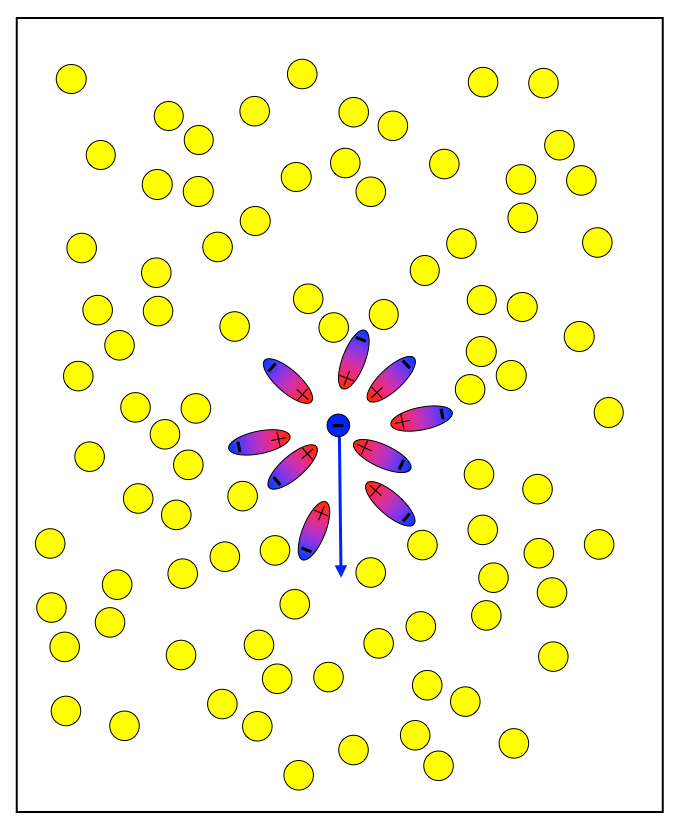
\includegraphics[width=\textwidth]{dipole_slow}
    \caption{$v < \frac{c}{n}$}
    \label{fig:dipole_slow}
  \end{subfigure}
  \hfill
  \begin{subfigure}[b]{0.49\textwidth}
    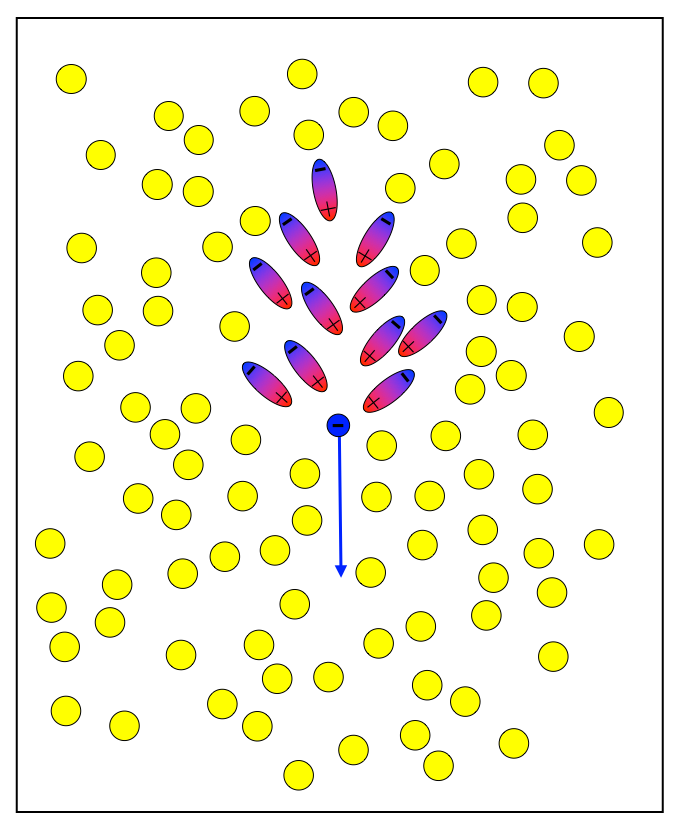
\includegraphics[width=\textwidth]{dipole_fast}
    \caption{$v \ge \frac{c}{n}$}
    \label{fig:dipole_fast}
  \end{subfigure}
  \caption[Polarisation produced in a dielectric medium due to the presence of a charged particle.]{Polarisation produced in a dielectric medium due to the presence of a charged particle, for the cases of a non-relativistic and relativistic particle.}
\end{figure}

\begin{figure}
	\centering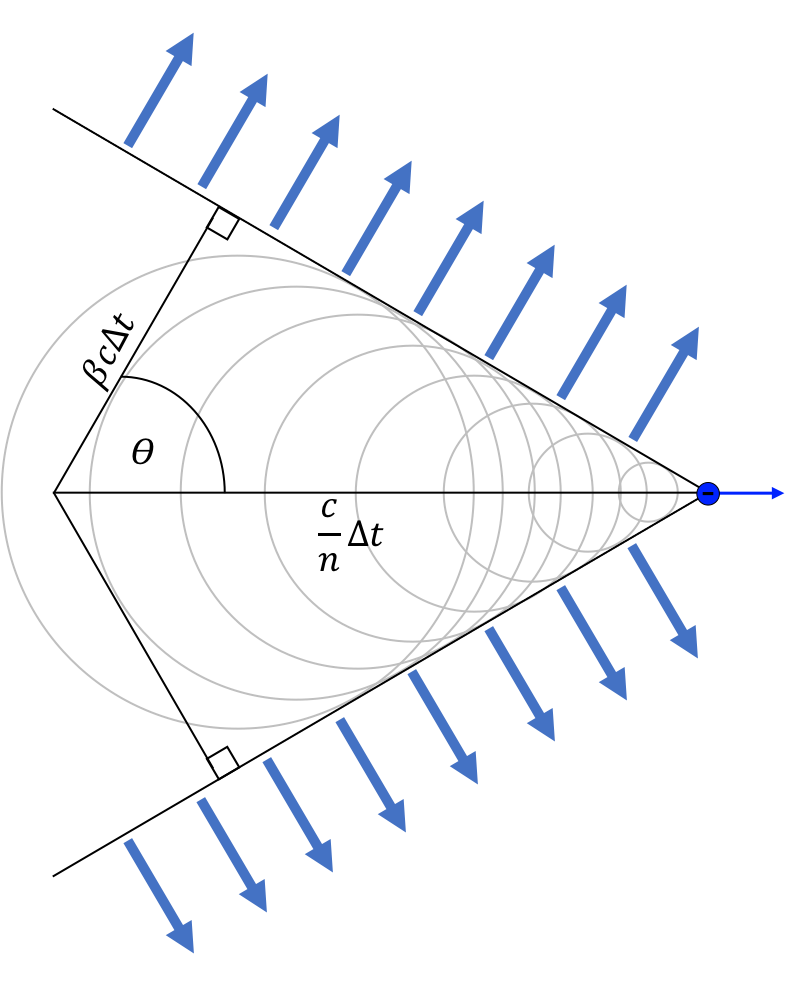
\includegraphics[width=0.5\textwidth]{cherenkov_geom} 
	\caption[Geometry of the wavefronts involved in Cherenkov radiation production.]{Geometry of the wavefronts involved in Cherenkov radiation production. The particle travels at a greater speed than the wavefronts propagate.}
	\label{fig:cherenkov_geom}
\end{figure}

When a charged particle moves slowly through a dielectric medium, the electric field of the particle distorts the nearby atoms. Momentarily, these atoms are transformed into elementary dipoles where the charged particles that constitute the atom are arranged with respect to the electric field of the travelling particle (Figure~\ref{fig:dipole_slow}). Due to the complete symmetry of this polarisation around the travelling particle, no net field is produced by the dielectric medium. However, if instead the velocity of the charged particle is faster than the speed light travels in that medium, an asymmetry along the particle trajectory is formed in the polarisation of the surrounding atoms (Figure~\ref{fig:dipole_fast}), resulting in a net dipole field. As the particle continues through the medium, elements of the polarised medium will release a brief burst of electromagnetic radiation. Generally these electromagnetic waves interfere destructively, except inside in the forward direction along the particles trajectory in an opening angle $\theta$. Although the full characterisation of this relativistic effect is complex, a simple consideration of the geometry involved, shown in Figure~\ref{fig:cherenkov_geom}, can be used to describe $\theta$ \cite{Jelley1958a}. In a time $\Delta t$ a particle travels a distance $\beta c \Delta t$ where $\beta = \frac{v}{c}$, while the emitted light will travel a distance $\frac{c}{n} \Delta t$ in a medium with refractive index $n$. This results in the relation:
\begin{equation} \label{eq:cherenkov_angle}
\cos \theta = \frac{vn}{c}.
\end{equation}
The blue light emitted in this constrained opening angle, via this phenomena, is known as Cherenkov radiation.

\section{Atmospheric Cherenkov Showers} \label{section:cherenkov_shower_intro}

\begin{figure}
	\centering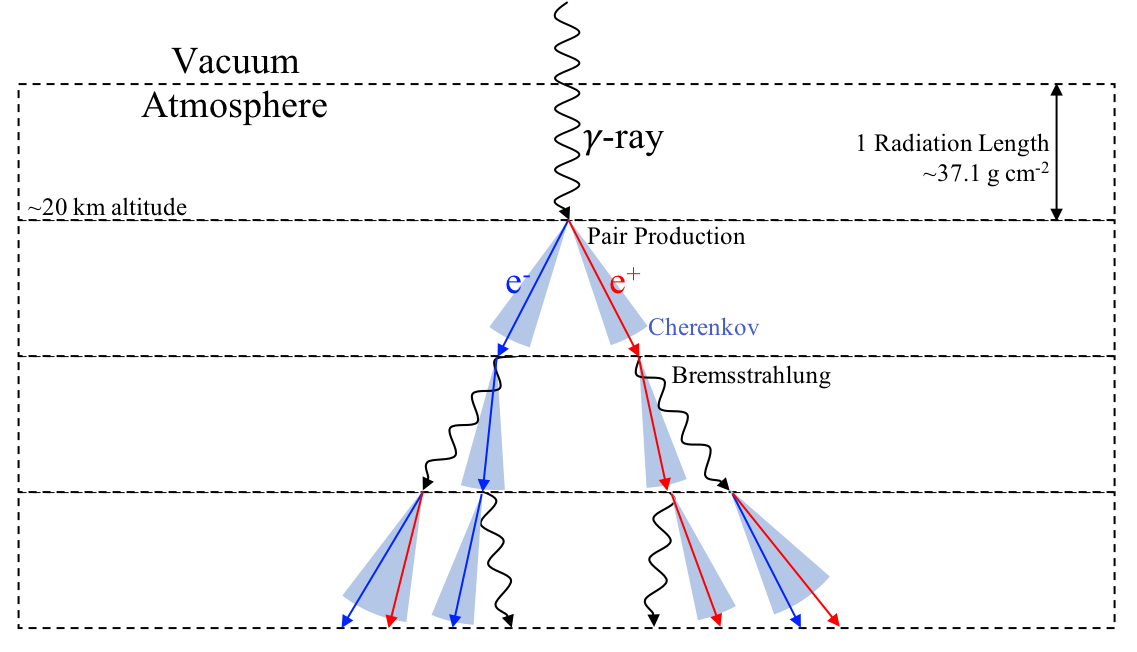
\includegraphics[width=\textwidth]{cascade} 
	\caption[Production of a extended electromagnetic particle cascade.]{Production of a extended electromagnetic particle cascade, demonstrating the different components and interactions.}
	\label{fig:cascade}
\end{figure}

The Earth's atmosphere is effectively opaque to photon energies above \SI{10}{eV} \cite{Weekes2003}. To conduct astronomical observations at higher energies, one must usually leave the Earth's atmosphere. However, at energies above \SI{\ge 10}{GeV}, a ``gamma-ray window'' exists where the pursuit of gamma-ray observations can be performed using the Cherenkov radiation produced by the cascade of particles resulting from the interaction between the gamma ray and the atmosphere.

Two electromagnetic interactions are responsible for the creation of this cascade:
\begin{description}
\item [Pair Production] The conversion of a photon into an electron-positron pair in the presence of an atom (such as an atmospheric particle). The energy of the photon must exceed the sum of the rest masses of an electron and positron (\SI{1.022}{MeV}). The electron-positron pair share the energy of the progenitor photon, and continue on a similar trajectory. This is the dominating interaction process for photons above \SI{\ge 10}{MeV} \cite{Weekes2003}.
\item [Bremsstrahlung radiation] The emission of a photon due to the interaction of a charged particle with the electric field on an atom (such as an atmospheric particle). This process allows further gamma rays to be produced.
\end{description}
The interplay between these two processes, occurring after each transversal of a radiation length, produces the extensive cascade of energetic electromagnetic particles. This is illustrated in Figure~\ref{fig:cascade}. The charged particles produced by the pair production in this cascade are responsible for the generation of the Cherenkov light. This cascade is often known as a ``Cherenkov shower''.

This cascade continues until the ionisation energy losses are equal to the radiation losses. The number of remaining particles after this point, known as the ``shower maximum'', begins to diminish. For a \SI{1}{TeV} shower this occurs at \SI{\sim 8.4}{km} altitude~\cite{Weekes2003}. The produced Cherenkov light is collimated along the progenitor gamma ray trajectory, and produces a pool of blue light on the ground, with a radius of \SI{\sim 120}{m}~\cite{Hillas1996a}. If the direction of the Cherenkov shower is extrapolated back to the cosmic sphere, the location of the source that produced the gamma ray can be inferred. Although the amount of energy that goes into Cherenkov photon production is a tiny fraction of the total energy, the atmosphere acts as a consistent calorimeter, therefore allowing an accurate reconstruction of the progenitors energy from the amount of Cherenkov photons produced. 

A further characteristic of the Cherenkov shower is the time profile. The entire shower typically lasts \SI{\sim 5}{ns}. Therefore, despite the abundance of showers in the sky, and the visible wavelength of the Cherenkov light, they are imperceivable by the human eye. Furthermore, due to the faster-than-light velocities of the particles inside the cascade, the last Cherenkov photons produced at the end of the shower reach the ground before the first Cherenkov photons produced at the start of the shower. With different sections of the showers arriving at different times, the Cherenkov shower measurements display a time gradient across the image. 

\section{Imaging Atmospheric Cherenkov Telescopes}

A primary issue in \gls{vhe} astronomy is the low flux (${\sim} 0.2$ per \si{m \squared} per year \cite{Franco2016}), requiring a collection area that is not feasible for space telescopes. If instead the Cherenkov showers are used to detect the gamma rays, large arrays of optical telescopes can be built to provide stereoscopic imaging of the Cherenkov showers. These telescopes are known as \glspl{iact}. The multiple stereoscopic views of individual showers provided by arrays of \glspl{iact} allow accurate reconstruction of the properties of the shower, such as direction and energy. The topic of reconstruction is discussed in Chapter~\ref{ch6-reduction}.

As the \gls{iact} technique involves imaging the Cherenkov showers, which are much larger than typical astronomy targets, \glspl{iact} do not require the resolving power of typical optical telescopes. Instead the priorities of an \gls{iact} optical system are to maximise: 
\begin{itemize}
\item Mirror collection area, such that more photons can be collected. This enables fainter showers to be detected, thereby lowering the energy threshold.
\item \gls{fov}, which improves the surveying capabilities and eases the study of extended sources.
\end{itemize}
Furthermore, the large collection area provided by the light pool of the Cherenkov shower enables a modest telescope to still make a large amount of gamma ray detections, enabling this technique to be viable despite the small flux.

\begin{figure}
	\centering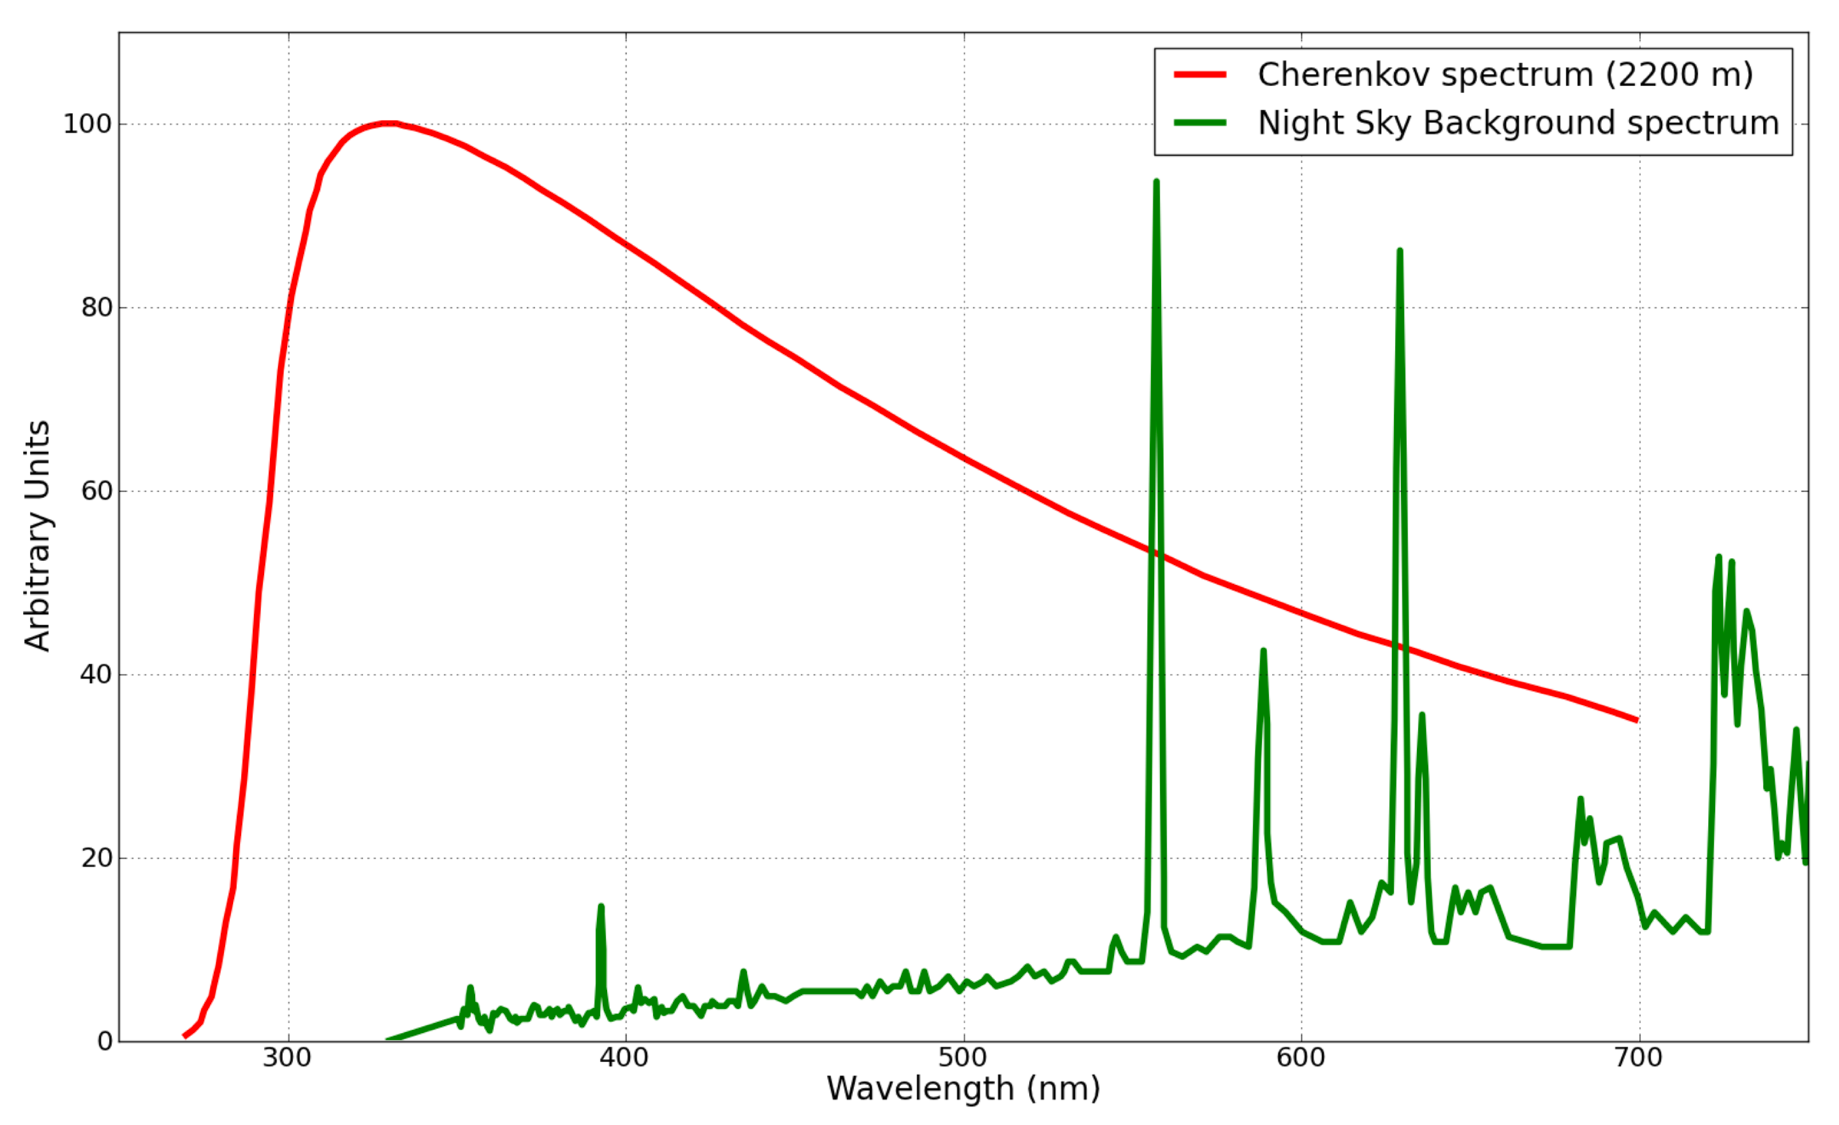
\includegraphics[width=\textwidth]{nsb} 
	\caption[Comparison of Cherenkov and NSB spectrum.]{Comparison of Cherenkov and NSB spectrum. The Cherenkov spectrum shown is expected at an altitude of \SI{2200}{m}. The NSB spectrum shown was measured at La Palma \cite{Bouvier2013}.}
	\label{fig:nsb}
\end{figure}

Two major background components need to be accounted for in \glspl{iact}:
\begin{description}
\item [Cosmic Ray Background] Protons (and heavier hadronic nuclei) are also capable of producing Cherenkov showers that are not entirely dissimilar to electromagnetic showers. As these particles are charged, they have been deflected by interstellar magnetic fields on their journey from their source, and therefore are not useful for \glspl{iact}. Therefore, these showers provide an isotropic background which is 1,000 times as numerous than the shower rate received from the discreet gamma-ray sources. However, a hadronic shower exhibits a morphology that is broader and less symmetric than that obtained from gamma-ray showers. Additionally, distinct features such as ``muon rings'', produced by highly penetrating muons reaching low altitudes such that the full Cherenkov cone is visible in a single telescope, accompany hadronic showers. Parametrisations of the Cherenkov shower image therefore enable the discrimination of the hadronic showers (see Chapter~\ref{ch6-reduction}. \change{images?}
\item [Night Sky Background] Due to the optical sensitivity of the cameras used by \glspl{iact}, the measurements taken are susceptible to starlight, moonlight, and artificial light pollution. The \gls{nsb} spectrum for La Palma, compared to the expected Cherenkov spectrum at an altitude of \SI{2200}{m}, is displayed in Figure~\ref{fig:nsb}. This background is excluded in two ways. Firstly, smart trigger logic and strict thresholds (such as the one described in Chapter~\ref{ch2-mechanics}) eliminate the triggering on \gls{nsb} photons. Secondly, unbiased charge extraction technique (described in Chapter~\ref{ch6-reduction}) exclude this noise from the signal.
\end{description}

The application of the \gls{iact} technique was first attempted in the 1960s, but the first large optical reflector built with the purpose of gamma-ray astronomy was the Whipple 10 m telescope in southern Arizona, 1968. At first, gamma-ray astronomy was polluted with unsubstantial claims of transient signals from a variety of pulsars and binaries, but these signals had marginal statistical significance \cite[][p.~9]{Weekes2003}. It wasn't until 20 years later, after further development of the technique, that the Crab Nebula was detected by Whipple in 1989, thus reigniting interest in the development of gamma-ray astronomy.

\begin{figure}
  \centering
  \begin{subfigure}[b]{0.35\textwidth}
  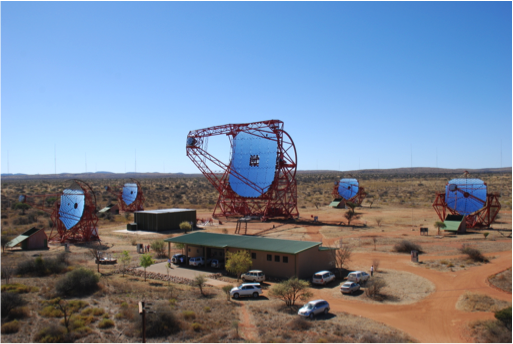
\includegraphics[width=\textwidth]{hess}
  \caption{H.E.S.S.}
  \label{fig:hess}
  \end{subfigure}
  ~
  \begin{subfigure}[b]{0.35\textwidth}
  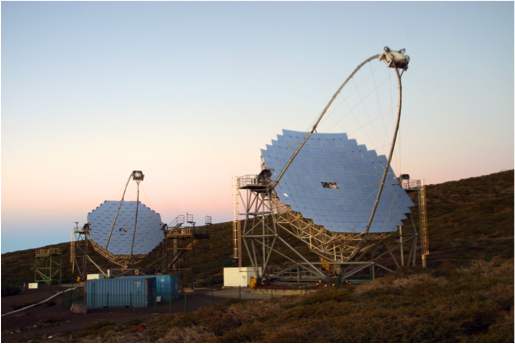
\includegraphics[width=\textwidth]{magic}
  \caption{MAGIC}
  \label{fig:magic}
  \end{subfigure}
  ~
  \begin{subfigure}[b]{0.45\textwidth}
  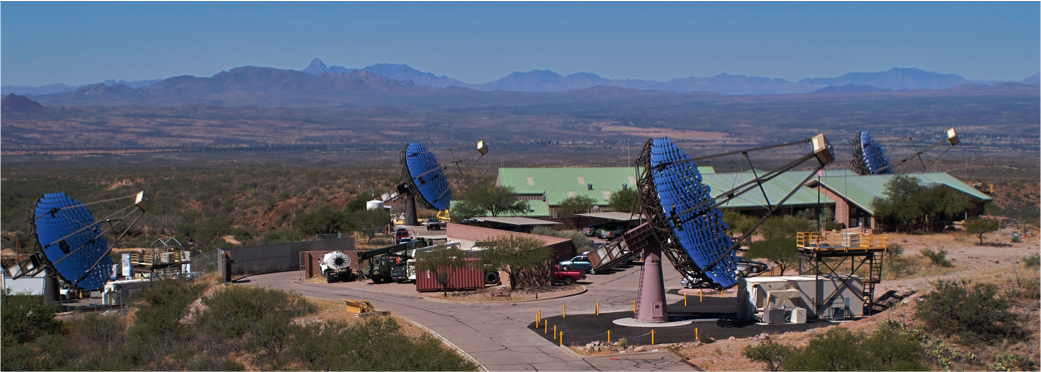
\includegraphics[width=\textwidth]{veritas}
  \caption{VERITAS}
  \label{fig:veritas}
  \end{subfigure}
  \caption{Photos of modern \glspl{iact}.}
  \label{fig:iacts}
\end{figure}

\begin{figure}
	\centering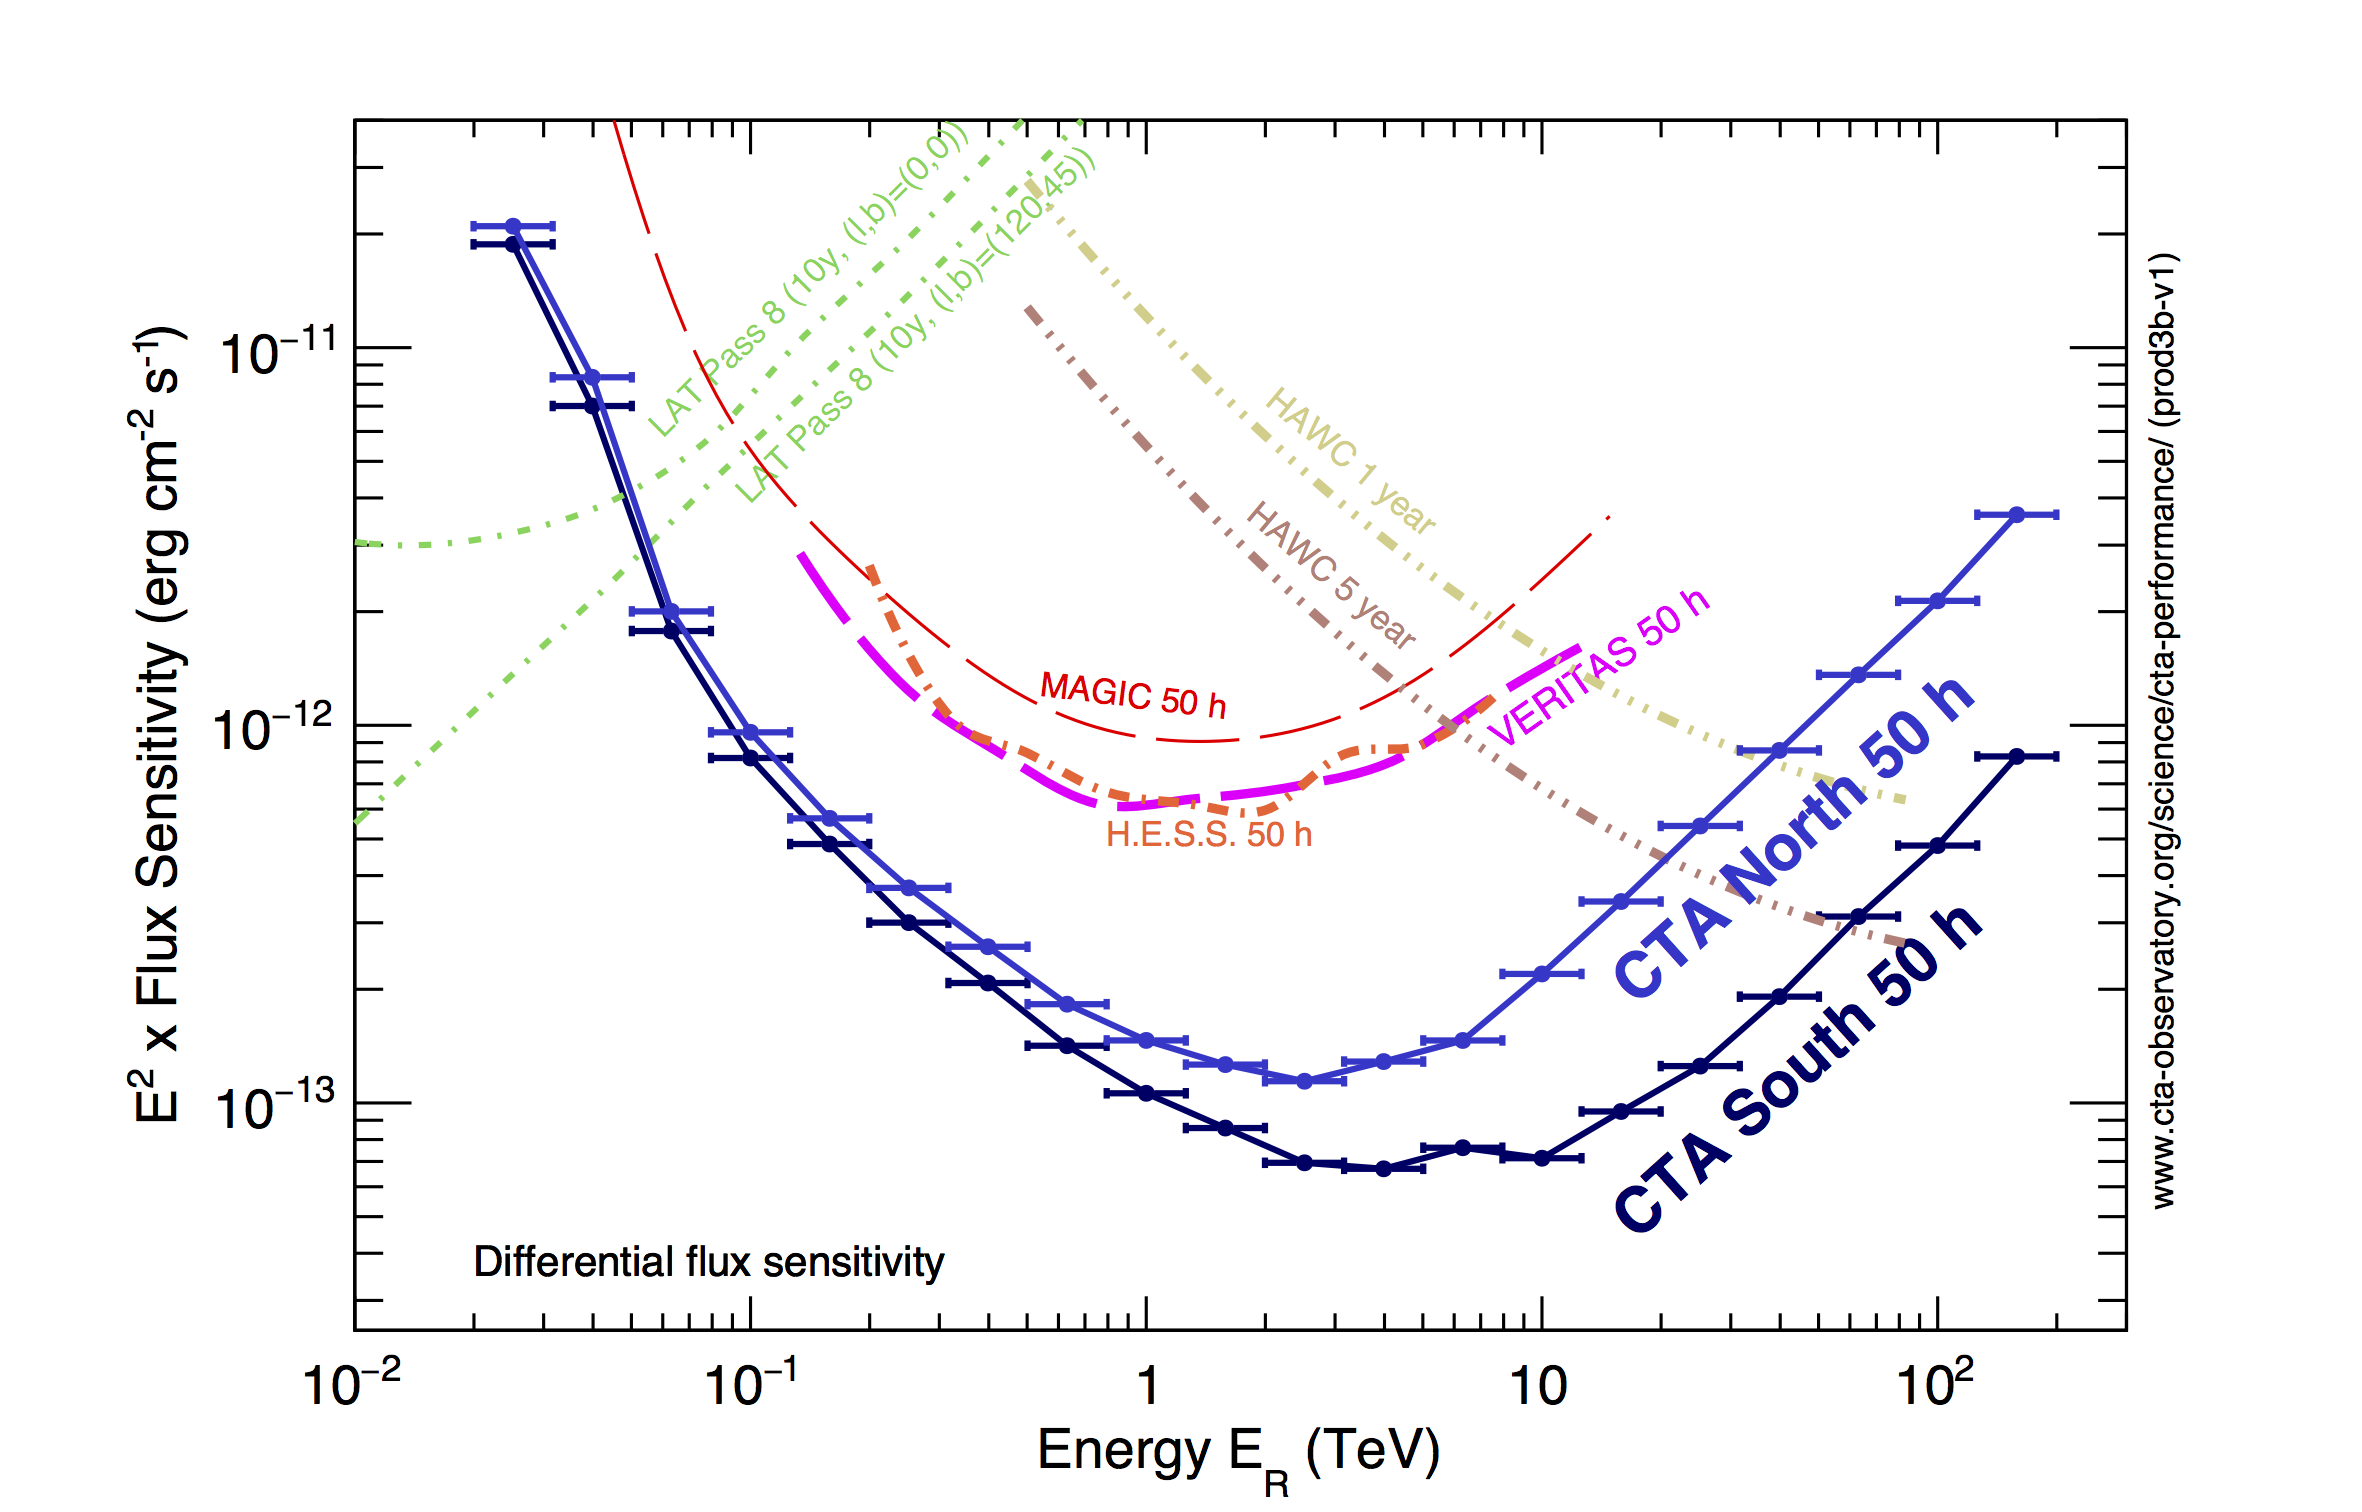
\includegraphics[width=\textwidth]{sensitivity} 
	\caption[Differential sensitivity of CTA.]{Differential sensitivity of CTA predicted by Monte Carlo simulations, compared to the performance of other gamma-ray instruments \cite{cta-performance}. The differential sensitivity has been defined as the minimum flux needed by CTA to obtain a 5-standard-deviation detection of a point-like source.}
	\label{fig:sensitivity}
\end{figure}

Modern \glspl{iact} include \gls{magic}, \gls{veritas}, and the most recent, \gls{hess} (Figure~\ref{fig:iacts}). All three of these telescope systems operate with the advantage of stereoscopic collaboration. In order to improve on the current \glspl{iact}, an array of ${\sim} 100$ telescopes was proposed, called the \gls{cta}. This array will have \cite{Acharya2013}:
\begin{itemize}
\item an improved sensitivity of 10 times over previous \glspl{iact} (Figure~\ref{fig:sensitivity}),
\item an observable gamma-ray energy range of \SI{30}{GeV} to \SI{100}{TeV},
\item a large (\SI{\sim 8}{\degree}) field of view for surveys,
\item improved angular and energy resolution,
\item and will be the first \gls{iact} to operate as an open observatory.
\end{itemize}

\section{The Cherenkov Telescope Array}

\begin{figure}
	\centering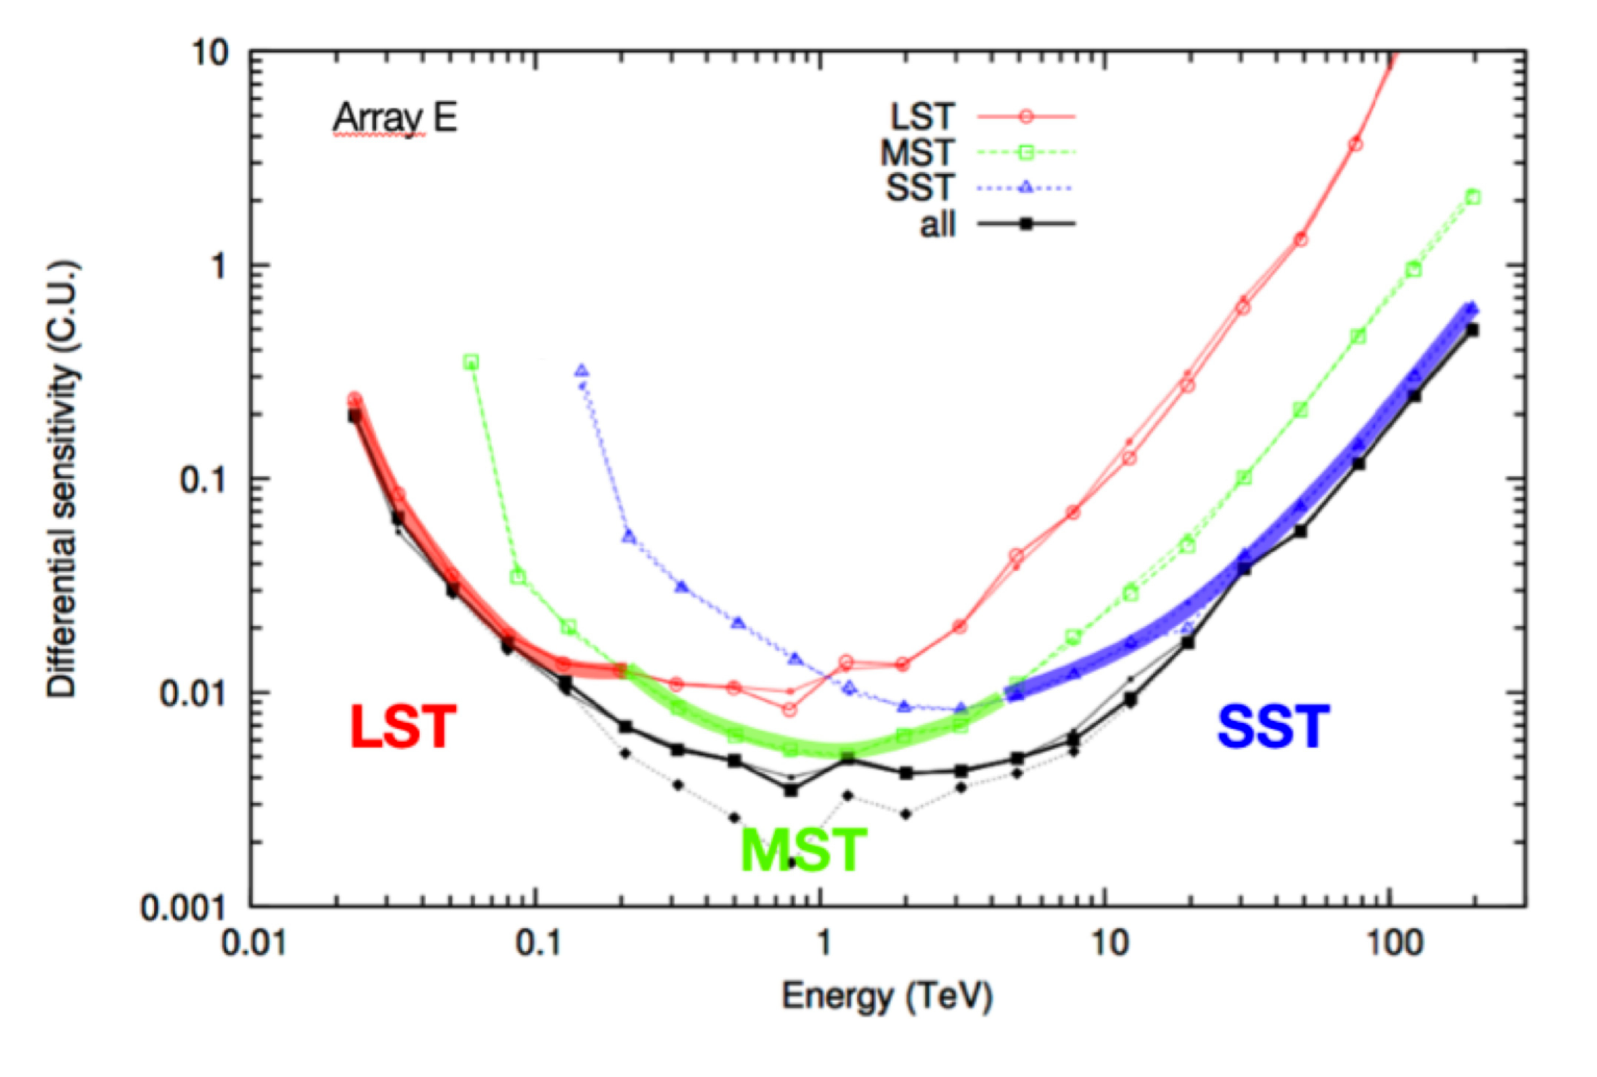
\includegraphics[width=\textwidth]{sensitivity_tel} 
	\caption[Differential sensitivity of the different CTA telescope types.]{Contribution of each telescope type within \gls{cta} to the total differential sensitivity \cite{Marano2014}.}
	\label{fig:sensitivity_tel}
\end{figure}

\gls{cta} will consist of three different sized telescopes:
\begin{itemize}
\item The \gls{lst}, with a mirror diameter of about \SI{23}{m} to enable the collection of as many photons as possible from the low energy showers (\SIrange{20}{150}{GeV}).
\item The \gls{mst}, covering the mid-range \SIrange{0.1}{10}{TeV} with mirror diameters of \SI{12}{m}.
\item The \gls{sst}, monitoring the high energies of \SIrange{1}{300}{TeV}, with mirror diameters of around \SI{4}{m}. Due to the rarity of higher energy showers, many \glspl{sst} need to be spread over an area of several square kilometres, to increase the chance of a detection \cite{Acharya2013}.
\end{itemize}
To illustrate these descriptions, the contributions of each telescope to the sensitivity of \gls{cta} is demonstrated in Figure~\ref{fig:sensitivity_tel}.

\begin{figure}
	\centering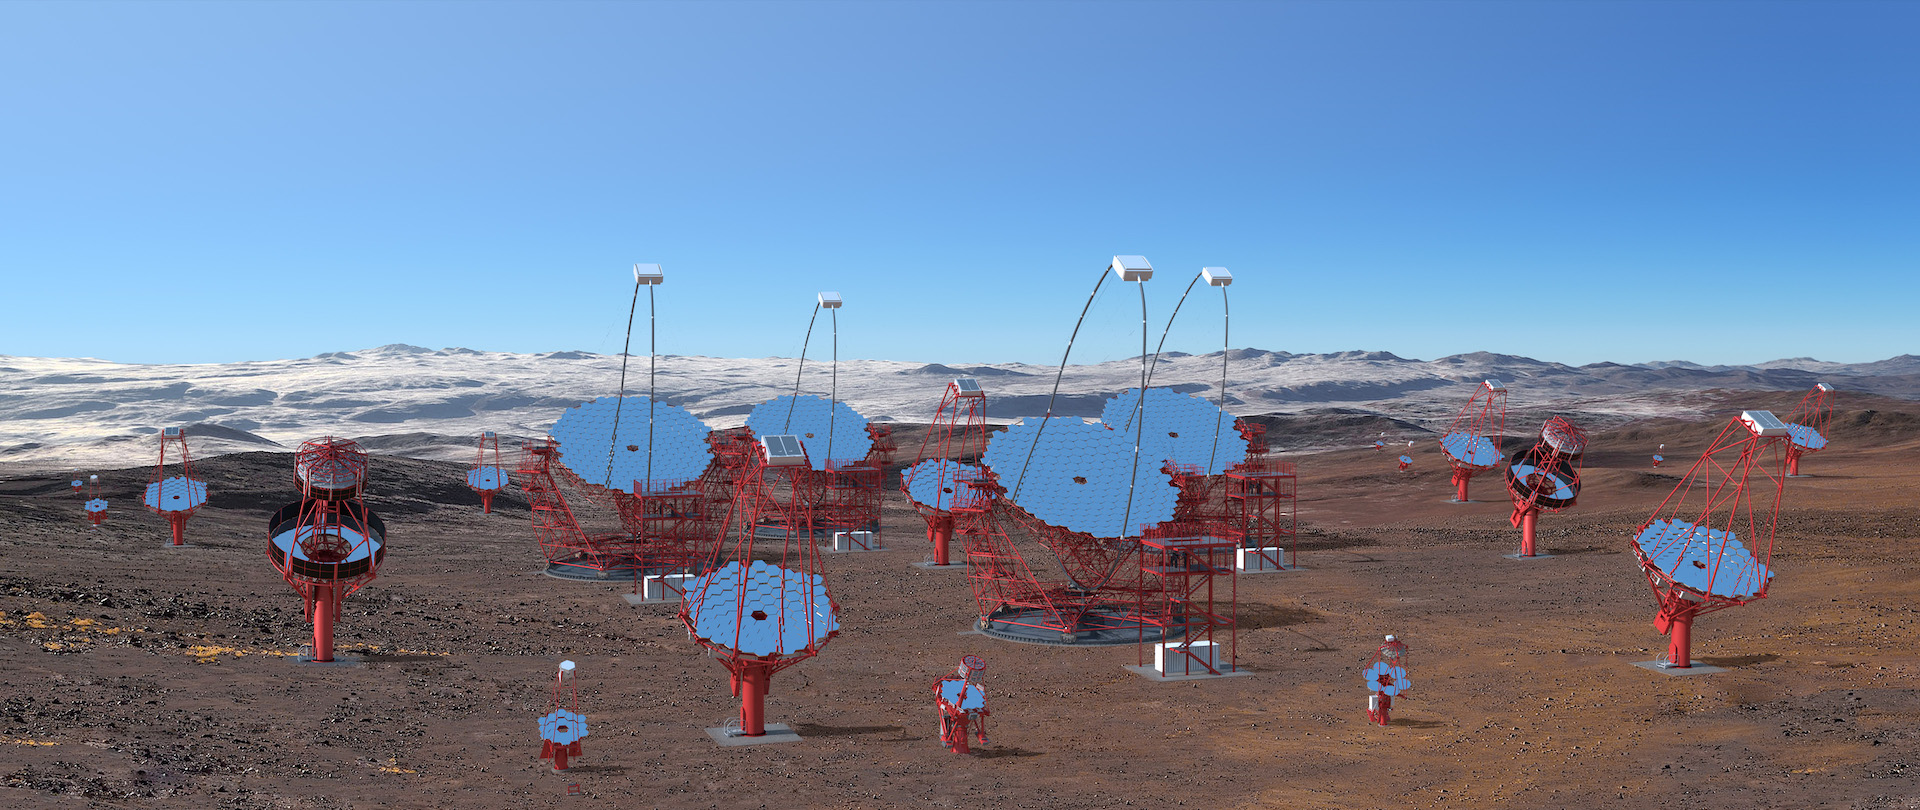
\includegraphics[width=\textwidth]{cta_south} 
	\caption[The southern-hemisphere Cherenkov Telescope Array.]{Computer-rendered graphic of the southern hemisphere site for the CTA three SST designs: GCT, ASTRI and SST-1M \cite{cta-sst}.}
	\label{fig:cta_south}
\end{figure}

Two \gls{cta} sites will exist. A northern hemisphere site for extragalactic observations will be built at La Palma, and is planned to contain 4 \glspl{lst} and 16 \glspl{mst}. As this site will focus on the energy range from \SI{20}{GeV} to \SI{20}{TeV}, no \glspl{sst} are included on the northern site. A southern hemisphere site will provide observations of the galactic plane, spanning the full energy range of \gls{cta}. Planned to be built nearby the Paranal Observatory in the Atacama Desert in Chile, the southern array is intended to feature 4 \glspl{lst}, 15 \glspl{mst}, and 70 \glspl{sst}, spread over \SI{4}{km \squared}. A visualisation of the \gls{cta} southern array is shown in Figure~\ref{fig:cta_south}.

\section{Small-Sized Telecopes}

\begin{figure}
	\centering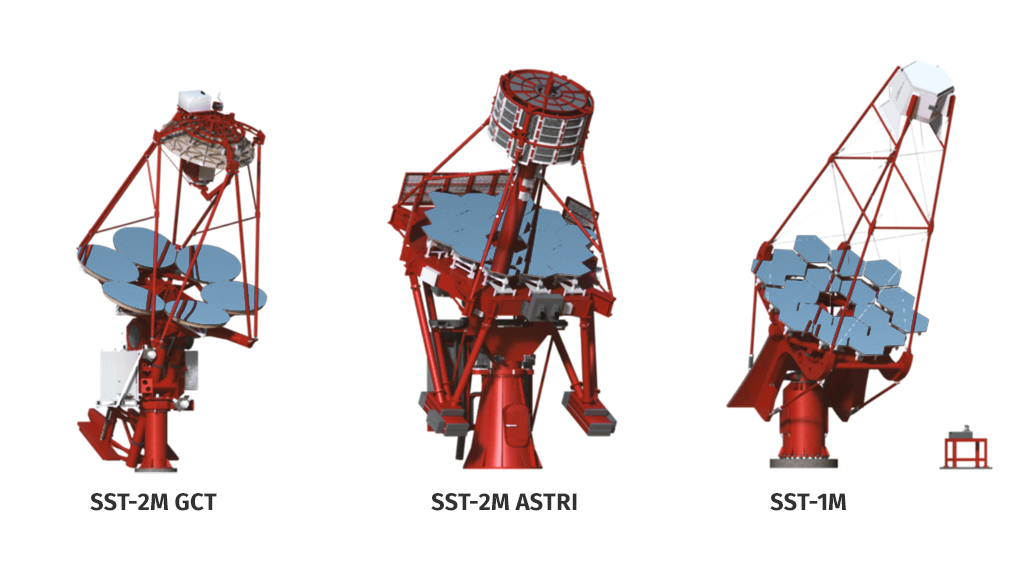
\includegraphics[width=\textwidth]{ssts} 
	\caption[The three SST designs.]{Computer-rendered graphics of the three SST designs: GCT, ASTRI and SST-1M \cite{cta-sst}.}
	\label{fig:ssts}
\end{figure}

Three designs for an \gls{sst} have been proposed:
\begin{itemize}
\item The SST-1M design, a single-mirror Davies-Cotton telescope developed in the colaboration between the Czech Republic, Ireland, Poland, Switzerland and Ukraine. The prototype structure was installed at the Institute of Nuclear Physics in Kraków, Poland in November 2013.
\item The \gls{astri} design features a dual-mirror Schwarzschild-Couder telescope structure. \gls{astri} is predominantly developed by Italy, however contributions were provided from Brazil and South Africa \cite{cta-sst}. The \gls{astri} prototype completed construction on Mt. Etna, Italy in 2014.
\item The \gls{gct} design also features a dual-mirror Schwarzschild-Couder telescope structure. \gls{gct} is being developed through collaboration between Australia, France, Germany, Japan, the Netherlands and the United Kingdom. The prototype telescope structure was inaugurated at the Observatoire de Paris-Meudon, France in November 2015. \gls{gct} is the telescope I have been associated with during my DPhil.
\end{itemize}
Visuals of all three telescopes are shown in Figure~\ref{fig:ssts}.

The Schwarzschild-Couder optical design was first proposed by German astrophysicist Karl Schwarzschild to eliminate optical aberrations across the \gls{fov}. This optical design has since gone through many interations, however it was never utilised for a reflector telescope due to the complexity and cost required to construct the mirrors \cite{Giro2017}. However, interest in the optical design was recently revitalised by \textcite{Vassiliev2007}, especially as it enables the utilisation of novel compact photosensors. Due to the same adoption of Schwarzschild-Couder optics, the telescopes of \gls{astri} and \gls{gct} have been specifically designed to accomodate the cameras from both \glspl{sst}. This increases the possibilities for the final \gls{sst} design for \gls{cta}.

\section{Science with the SSTs}

As shown in Figures~\ref{fig:sensitivity}~and~\ref{fig:sensitivity_tel}, the \glspl{sst} are responsible for exploring beyond the current energy frontier in gamma-ray astronomy. Within 50 hours, the \glspl{sst} will be able provide the same sensitivity as five years of observations with the \gls{hawc} observatory \cite{Consortium2018}. This enables \gls{cta} to provide insights into the most energetic processes in the universe, and address prevalant topics of debate in \gls{vhe} astronomy and particle phyiscs.

The high energy science cases of \gls{cta} are mostly concerned with the acceleration mechanisms that produce high energy cosmic rays. This has been an active topic of discussion in the past 100 years since their initial detection. It is therefore hoped that the \gls{cta} \glspl{sst} can provide new insights into these mechanisms. The different investigations related to this topic can be loosly consolidated into the following catagories:
\begin{description}
\item [Supernova Remnants] It is known that the galactic population of \glspl{snr} play an important role in the accelaration of cosmic rays to high energies. The detection of \si{TeV} photons from \glspl{snr} (suggesting an efficient acceleration mechanism), and the description of the diffusive shock acceleration mechanism, both corraborate with the detection of high-energy cosmic rays in the Earth's atmosphere \cite{Cristofari2017}. However, the detection of \si{TeV} photons from \glspl{snr} could instead be explained by the inverse-Compton scattering betweeen accelerated electrons and the ambient photon background. Therefore, the debate between a leptonic or hadronic origin is still ongoing \cite{Acharya2013}. While studies of individual \glspl{snr} have improved our understanding of the acceleration mechanisms, a population wide study may help constrain the parameters involved \cite{Cristofari2017}. The probe into higher energies with the \glspl{sst} will provide further information about the spectral energy distribution of the currently known \glspl{snr}, and the enhanced sensitivity of \gls{cta} will increase the population of \glspl{snr} known to emit at these energies.
\item [Origin of Cosmic Rays] Another important question regarding the locally measured flux of high-energy cosmic rays is their origin \cite{Bigongiari2016}. As just described, \glspl{snr} do appear to be a dominant source for these particles, but are they the only major contributor to the galactic cosmic rays? Expanding on the discovered \gls{vhe} galactic source population is the key to answering this question.
\item [Pevatrons] A further capability of \gls{cta} (provided by the \glspl{sst}) is the detection of extreme accelerators that power particles up to the \si{PeV} scale. As a result of the acceleration of hadronic cosmic rays to these energies, gamma rays with energies of /SI{100}{TeV} should be detectable from the accelerator. However, as the cross-section for inverse-Compton electron-photon interactions decreases very quickly above a few tens of \si{TeV} \cite{Consortium2018}, the absense of /SI{100}{TeV} gamma rays from these accelerators would suggest a leptonic origin. The identification of even one Pevatron acccelerator would therefore provide a huge breakthrough in the inevfffsfdstigtions into

and allow us to understand the physics of the most extreme accelerators in the Galaxy.

The preferential production of \SI{100}{TeV} photons by hadronic processes will be paramount in disentagling the ``problematic ambiguity between leptonic and hadronic origin'' of \gls{vhe} gamma rays \cite[][p. 132]{Consortium2018}.
\end{description}
%\begin{savequote}[8cm]
%Alles Gescheite ist schon gedacht worden.\\
%Man muss nur versuchen, es noch einmal zu denken.
%
%All intelligent thoughts have already been thought;\\
%what is necessary is only to try to think them again.
%  \qauthor{--- Johann Wolfgang von Goethe \cite{von_goethe_wilhelm_1829}}
%\end{savequote}

\chapter{\label{ch:2-litreview}Background}

\minitoc

\section{Introduction}

This document introduction won't serve as a complete primer on \LaTeX.  There are plenty of those online, and googling your questions will often get you answers, especially from \url{http://tex.stackexchange.com}.

Instead, let's talk a little about a few of the features and packages lumped into this template situation.  The \verb|savequote| environment at the beginning of chapters can add some wittiness to your thesis.  If you don't like the quotes, just remove that block.

For when it comes time to do corrections, there are two useful commands here.  First, the \verb|mccorrect| command allows you to highlight a short correction \mccorrect{like this one}.  When the thesis is typeset normally, the correction will just appear as part of the text.  However, when you declare \verb|\correctionstrue| in the main \verb|Oxford_Thesis.tex| file, that correction will be highlighted in blue.  That might be useful for submitting a post-viva, corrected copy to your examiners so they can quickly verify you've completed the task.

\begin{mccorrection}
For larger chunks, like this paragraph or indeed entire figures, you can use the \verb|mccorrection| environment.  This environment highlights paragraph-sized and larger blocks with the same blue colour.
\end{mccorrection}

Read through the \verb|Oxford_Thesis.tex| file to see the various options for one- and two-sided printing, including or excluding the separate abstract page, and turning corrections and draft footer on or off, and the separate option to centre your text on the page (for PDF submission) or offset it (for binding).  There is also a separate option for master's degree submissions, which changes identifying information to candidate number and includes a word count.  (Unfortunately, \LaTeX has a hard time doing word counts automatically, so you'll have to enter the count manually if you require this.)

\section{Cardiac Imaging}\label{app:imaging}

Within months of Röntgen's discovery of the X-ray in \mccorrect{1895}\cite{gagliardi_rontgen_1996}, cardiac pathology was being investigated via non-invasive imaging \cite{gagliardi_cardiac_1996}.  Over the intervening years, cardiac imaging modalities and techniques have advanced significantly.  Clinically, cardiac imaging is used for two broad purposes: diagnosis of pathophysiology and guidance of interventional procedures.  These applications impose different requirements on imaging equipment, image acquisition time, computational complexity, spatial and temporal resolution, and tissue discrimination.  The common diagnostic and interventional cardiac imaging techniques in current clinical practice are reviewed below.  An accessible introduction to the physics of medical imaging can be found in Webb's \textit{Introduction to Biomedical Imaging} \cite{webb_introduction_2002}.  A comprehensive overview of the use of imaging in clinical cardiology is presented in Leeson's \textit{Cardiovascular Imaging} \cite{leeson_cardiovascular_2011}.

\subsection{Diagnostic Imaging}
\label{sub:diagnostic}

Beyond the chest X-ray (`plain film'), the key non-invasive imaging modalities in diagnostic cardiology are echocardiography, magnetic resonance imaging, and X-ray computed tomography, which are reviewed below.  Nuclear medicine, including positron emission tomography (PET) and single-photon emission computed tomography (SPECT), are not discussed here, as they do not play a role in the chapters to follow.

\subsubsection{Echocardiography}

\begin{figure}
\centering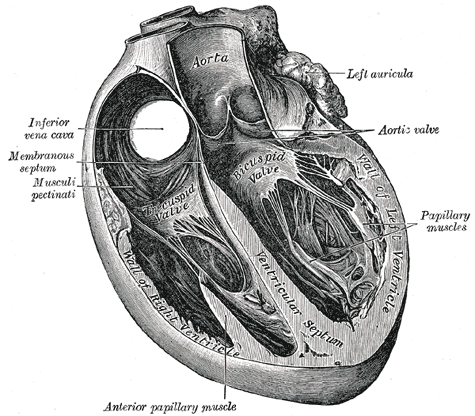
\includegraphics[width=0.7\textwidth]{figures/sample/Gray498.png} 
\caption[Four-chamber illustration of the human heart.]{Four-chamber illustration of the human heart.  Clockwise from upper-left: right atrium, left atrium, left ventricle, right ventricle.}
\label{fig:fourchamber}\end{figure}

The use of acoustic waves for medical diagnosis, inspired by naval sonar, was initially developed in the 1940s \cite{gagliardi_ultrasonography_1996}.  By 1954, the first clinically useful cardiac ultrasound -- examining motion of the mitral valve in stenosis -- was reported \cite{edler_ultrasonic_1957}.  These early scans were one-dimensional images (`A-mode'), sometimes repeated to generate a time axis (`M-mode').   The sector-scanning probe was developed in the 1970s \cite{bom_ultrasonic_1971,griffith_sector_1974}, leading to the `B-mode' that a modern cardiologist would recognise as an echocardiogram.



%% APPENDICES %% 
% Starts lettered appendices, adds a heading in table of contents, and adds a
%    page that just says "Appendices" to signal the end of your main text.
\startappendices
% Add or remove any appendices you'd like here:
\chapter{\label{app:1-cardiophys}Review of Cardiac Physiology and Electrophysiology}

\minitoc

Appendices are just like chapters.  Their sections and subsections get numbered and included in the table of contents; figures and equations and tables added up, etc.  Lorem ipsum dolor sit amet, consectetur adipiscing elit. Sed et dui sem. Aliquam dictum et ante ut semper. Donec sollicitudin sed quam at aliquet. Sed maximus diam elementum justo auctor, eget volutpat elit eleifend. Curabitur hendrerit ligula in erat feugiat, at rutrum risus suscipit. Pellentesque habitant morbi tristique senectus et netus et malesuada fames ac turpis egestas. Integer risus nulla, facilisis eget lacinia a, pretium mattis metus. Vestibulum aliquam varius ligula nec consectetur. Maecenas ac ipsum odio. Cras ac elit consequat, eleifend ipsum sodales, euismod nunc. Nam vitae tempor enim, sit amet eleifend nisi. Etiam at erat vel neque consequat.

\section{Anatomy}
\label{sec:anatomy}

Lorem ipsum dolor sit amet, consectetur adipiscing elit. Donec accumsan cursus neque. Pellentesque eget tempor turpis, quis malesuada dui. Proin egestas, sapien sit amet feugiat vulputate, nunc nibh mollis nunc, nec auctor turpis purus sed metus. Aenean consequat leo congue volutpat euismod. Vestibulum et vulputate nisl, at ultrices ligula. Cras pulvinar lacinia ipsum at bibendum. In ac augue ut ante mollis molestie in a arcu.

Etiam vitae quam sollicitudin, luctus tortor eu, efficitur nunc. Vestibulum maximus, ante quis consequat sagittis, augue velit luctus odio, in scelerisque arcu magna id diam. Proin et mauris congue magna auctor pretium id sit amet felis. Maecenas sit amet lorem ipsum. Proin a risus diam. Integer tempus eget est condimentum faucibus. Suspendisse sem metus, consequat vel ante eget, porttitor maximus dui. Nunc dapibus tincidunt enim, non aliquam diam vehicula sed. Proin vel felis ut quam porta tempor. Vestibulum elit mi, dictum eget augue non, volutpat imperdiet eros. Praesent ac egestas neque, et vehicula felis.

Pellentesque malesuada volutpat justo, id eleifend leo pharetra at. Pellentesque feugiat rutrum lobortis. Curabitur hendrerit erat porta massa tincidunt rutrum. Donec tincidunt facilisis luctus. Aliquam dapibus sodales consectetur. Suspendisse lacinia, ipsum sit amet elementum fermentum, nulla urna mattis erat, eu porta metus ipsum vel purus. Fusce eget sem nisl. Pellentesque dapibus, urna vitae tristique aliquam, purus leo gravida nunc, id faucibus ipsum magna aliquet ligula. Lorem ipsum dolor sit amet, consectetur adipiscing elit. Proin sem lacus, rutrum eget efficitur sed, aliquam vel augue. Aliquam ut eros vitae sem cursus ultrices ut ornare urna. Nullam tempor porta enim, in pellentesque arcu commodo quis. Interdum et malesuada fames ac ante ipsum primis in faucibus. Curabitur maximus orci purus, ut molestie turpis pellentesque ut.

Donec lacinia tristique ultricies. Proin dignissim risus ut dolor pulvinar mollis. Proin ac turpis vitae nibh finibus ullamcorper viverra quis felis. Mauris pellentesque neque diam, id feugiat diam vestibulum vitae. In suscipit dui eu libero ultrices, et sagittis nunc blandit. Aliquam at aliquet ex. Nullam molestie pulvinar ex vitae interdum. Praesent purus nunc, gravida id est consectetur, convallis elementum nulla. Praesent ex dolor, maximus eu facilisis at, viverra eget nulla. Donec ullamcorper ante nisi. Sed volutpat diam eros. Nullam egestas neque non tortor aliquet, sed pretium velit tincidunt. Aenean condimentum, est ac vestibulum mattis, quam augue congue augue, mattis ultrices nibh libero non ante. Lorem ipsum dolor sit amet, consectetur adipiscing elit.

Aenean volutpat eros tortor, non convallis sapien blandit et. Maecenas faucibus nulla a magna posuere commodo. Nullam laoreet ante a turpis laoreet malesuada. Phasellus in varius sem. Vestibulum sagittis nibh sed tincidunt blandit. Donec aliquam accumsan odio sit amet lacinia. Integer in tellus diam. Vivamus varius massa leo, vitae ullamcorper metus pulvinar sed. Maecenas nec lorem ornare, elementum est quis, gravida massa. Suspendisse volutpat odio ex, ac ultrices leo ultrices vel. Sed sed convallis ipsum. Pellentesque euismod a nulla sed rhoncus. Sed vehicula urna vitae mi aliquet, non sodales lacus ullamcorper. Duis mattis justo turpis, id tempus est tempus eu. Curabitur vitae hendrerit ligula.

Curabitur non pretium enim, in commodo ligula. Etiam commodo eget ligula a lacinia. Vestibulum laoreet ante tellus, vel congue sapien ornare in. Donec venenatis cursus velit vitae pulvinar. Pellentesque habitant morbi tristique senectus et netus et malesuada fames ac turpis egestas. Suspendisse in metus lectus. Pellentesque gravida dolor eget finibus imperdiet. Duis id molestie tortor. Mauris laoreet faucibus facilisis. Aliquam vitae dictum massa, sit amet dignissim lacus.

Fusce eleifend tellus id ex consequat maximus. Donec ultrices ex ut turpis ornare, non molestie mi placerat. Nulla sit amet auctor nunc, sit amet euismod elit. Phasellus risus tellus, condimentum a metus et, venenatis tristique urna. Cras mattis felis eget ipsum fermentum egestas. Ut augue odio, venenatis id convallis vel, congue quis augue. Maecenas sed maximus est, posuere aliquet tortor. Ut condimentum egestas nisi eu porttitor. Ut mi turpis, posuere id lorem vel, elementum tempor arcu.

Morbi nisl arcu, venenatis non metus ac, ullamcorper scelerisque justo. Nulla et accumsan lorem. Mauris aliquet dui sit amet libero aliquet, in ornare metus porttitor. Integer ultricies urna eu consequat ultrices. Maecenas a justo id purus ultricies posuere sed et quam. Cum sociis natoque penatibus et magnis dis parturient montes, nascetur ridiculus mus. Sed eleifend risus quis aliquet gravida. Nullam ac erat porta est bibendum dictum in a dolor. Nam eget turpis viverra, vulputate lectus eget, mattis ligula. Nam at tellus eget dui lobortis sodales et ut augue. In vestibulum diam eget mi cursus, ut tincidunt nulla pellentesque.

Aliquam erat volutpat. Sed ultrices massa id ex mattis bibendum. Nunc augue magna, ornare at aliquet gravida, vehicula sed lorem. Quisque lobortis ipsum eu posuere eleifend. Duis bibendum cursus viverra. Nam venenatis elit leo, vitae feugiat quam aliquet sed. Cras velit est, tempus ac lorem sed, pharetra lobortis ipsum. Donec suscipit gravida interdum. Nunc non finibus est. Nullam turpis elit, tempus non ante.

\section{Mechanical Cycle}

Lorem ipsum dolor sit amet, consectetur adipiscing elit. Aenean tellus est, suscipit sed facilisis quis, malesuada at ipsum. Nam tristique urna quis quam iaculis, et mattis orci pretium. Praesent euismod elit vel metus commodo ultrices. Vestibulum et tincidunt ex, in molestie ex. Donec ullamcorper sollicitudin accumsan. Etiam ac leo turpis. Duis a tortor felis. Nullam sollicitudin eu purus ac hendrerit. Nam hendrerit ligula libero, eget finibus orci bibendum a. Aenean ut ipsum magna.

Ut viverra, sapien sed accumsan blandit, nisi sem tempus tellus, at suscipit magna erat ornare nunc. Proin lacinia, nisi ut rutrum malesuada, nibh quam pellentesque nunc, sit amet consectetur purus felis ac tortor. Suspendisse lacinia ipsum eu sapien pellentesque mattis. Mauris ipsum nunc, placerat non diam vel, efficitur laoreet nunc. Sed lobortis, ipsum eget gravida facilisis, sem nulla viverra mi, in placerat eros sem viverra lacus. Aliquam porta aliquet diam vel commodo. Nulla facilisi. Duis erat libero, lobortis vel hendrerit vitae, sagittis id dui. Nulla pretium eros nec quam tincidunt, vel luctus mi aliquam. Integer imperdiet purus in est tristique venenatis. Ut pellentesque, nunc vitae iaculis ultricies, urna turpis dignissim risus, a laoreet felis magna nec erat.

Quisque sollicitudin faucibus ligula, et egestas nibh dictum sit amet. Proin eu mi a lectus congue pretium eu quis arcu. Suspendisse vehicula libero eu ipsum aliquam, vel elementum nibh mattis. Sed sed sapien vitae turpis tristique pulvinar a ut metus. Etiam semper gravida est, mollis gravida est porta ac. Proin eget tincidunt erat. Maecenas ultrices erat eget purus ultricies, ut lacinia arcu dictum. Nam et nisi sit amet ex congue mattis vel eget lorem. Aliquam erat volutpat. Pellentesque porttitor nibh vitae elementum consectetur. Aenean et est lobortis, congue sapien non, ullamcorper sapien. Ut facilisis sem non dapibus vehicula.

Mauris euismod odio dolor, sit amet gravida mauris placerat et. Curabitur nec dolor non nibh molestie lobortis dignissim non ante. Nullam rutrum lobortis ultrices. Aenean ex erat, elementum sed maximus id, posuere id quam. Proin rutrum ex elit, pretium aliquam risus finibus at. Aenean egestas orci velit, sed aliquet sapien condimentum a. Duis consequat, arcu eu viverra venenatis, dolor lorem gravida lectus, non aliquet nisi sem at augue. Donec laoreet blandit luctus. Aenean vehicula nisl vel faucibus luctus. Sed ut semper velit, vitae laoreet magna. Sed at interdum magna.

Sed iaculis faucibus odio, eu aliquam purus efficitur vel. Cras at nulla ac enim congue varius ut et nulla. Integer blandit mattis augue.

\section{Electrical Cycle}
\label{sec:electcycle}

Lorem ipsum dolor sit amet, consectetur adipiscing elit. In faucibus condimentum rhoncus. Ut dictum nisl id risus gravida lobortis. Sed vehicula mollis tellus ut varius. Fusce eget egestas dui, et commodo dui. Proin sollicitudin interdum tempus. Nullam in elit a enim fringilla bibendum. Vestibulum sodales pellentesque condimentum. Nulla facilisi. Nunc et dolor in nulla eleifend dictum at vel ligula. Aliquam ut velit non elit ullamcorper porta ac et ex. Fusce ornare magna non nunc vestibulum, eget molestie quam dictum. In interdum aliquam odio, in posuere tellus convallis quis. Curabitur non diam elit. Proin vulputate orci diam, a tincidunt ante luctus eu. Ut a viverra ligula. Curabitur pulvinar tempus tellus eget suscipit.

Aliquam posuere massa at ante dapibus congue. Curabitur ullamcorper tortor eget consectetur aliquet. Mauris tempor magna id mauris fringilla, a varius erat blandit. Nam eleifend ullamcorper placerat. Phasellus augue tortor, volutpat bibendum lorem nec, fringilla volutpat nisl. Mauris cursus urna metus, vel eleifend orci iaculis ut. Sed sit amet scelerisque massa, quis consequat dui. Donec semper sem dui, ac placerat velit egestas vel. Nulla facilisi. Quisque tellus eros, sagittis malesuada augue ut, faucibus dictum nulla. Vestibulum non dapibus erat, ut consequat libero. Ut turpis mi, dapibus commodo libero lobortis, maximus vestibulum lectus. Vestibulum sit amet sapien dapibus, tincidunt leo in, suscipit arcu. Sed in erat bibendum, laoreet eros eu, pellentesque justo. Nulla sodales purus neque, eget maximus ipsum consequat at. Maecenas a nisl sagittis, tempus ipsum sed, dictum mauris.

Suspendisse posuere odio lacus, at auctor tortor vehicula sed. Phasellus suscipit ornare enim vitae placerat. Sed viverra purus vel sapien tempor, quis iaculis erat laoreet. Aenean vel nunc vestibulum, ornare nunc ac, mollis urna. Aenean ultrices felis ipsum, ac semper est ullamcorper in. Donec in justo varius, egestas tortor ut, venenatis augue. Duis mattis, ligula quis lacinia fringilla, tellus neque accumsan ipsum, vitae tempor metus elit vel nibh. Curabitur porttitor urna nec sapien tempor, et porttitor velit malesuada.

Suspendisse aliquam nisl quis placerat vulputate. Proin dapibus ipsum ac ante sagittis, volutpat auctor sem dapibus. Nam in facilisis odio. Integer ante mauris, eleifend et pulvinar in, venenatis quis ligula. Phasellus posuere sollicitudin tortor eget euismod. Maecenas mollis tortor eget justo vulputate sagittis. Etiam hendrerit massa quis ex molestie sodales. Quisque facilisis erat lacus, id convallis sem suscipit bibendum. Integer dui urna, pharetra sed porta sed, bibendum ut odio. Donec placerat at lectus egestas consequat. Sed id rhoncus est, vitae vulputate sapien. Fusce tempus quam lorem, id ornare turpis sodales sed. Integer aliquet urna eget condimentum consequat. Vestibulum quis dui vel ligula posuere luctus id nec turpis.

Nam vitae placerat lacus. Mauris scelerisque interdum volutpat. Nunc aliquet tristique enim, sit amet molestie felis ullamcorper vitae. Nullam sollicitudin orci orci, in condimentum tellus consectetur in. Nam id justo justo. Fusce eget finibus est. Proin id tortor nec quam cursus vehicula. Aliquam ultrices eros eros, a tincidunt elit eleifend auctor.

Nullam consectetur dapibus ligula sit amet efficitur. Nunc non posuere sapien. Vivamus dui nisl, aliquam id ipsum non, pulvinar ornare neque. Nunc rhoncus pretium congue. Fusce id laoreet enim. Cras sed massa in eros bibendum auctor in nec sem. Nam commodo, velit id porta consequat, mi arcu gravida lorem, ut aliquam elit ante quis dui. Quisque in massa sed nibh blandit dictum.

Vestibulum molestie consectetur porttitor. Donec tincidunt vel orci at pharetra. Nullam id felis sit amet nulla tempus lacinia. Integer egestas ullamcorper massa, ut ultricies diam congue sit amet. Cras sit amet velit at nibh vehicula finibus a et lorem. Cras odio metus, venenatis ut ultrices non, ornare ac orci. Morbi et nulla dui. Mauris dictum molestie nibh, eu efficitur lorem accumsan quis.

\section{Cellular Electromechanical Coupling}
\label{sec:electromech}

Lorem ipsum dolor sit amet, consectetur adipiscing elit. Nullam vitae consectetur metus, ac maximus ex. Quisque vitae ex eu lectus ultricies consequat vel non lorem. Etiam odio ipsum, tempus ut lobortis in, molestie ac leo. Vivamus mollis feugiat bibendum. Vestibulum eget venenatis quam. Aenean faucibus, massa sed ullamcorper porta, arcu nunc iaculis velit, quis consectetur purus neque placerat nibh. Vestibulum elit nunc, dignissim vulputate venenatis et, sodales non massa. Proin leo ligula, vehicula eu aliquam varius, posuere a dolor. Donec iaculis auctor neque, sit amet gravida libero porta vel. Vivamus consequat elementum lacus, at bibendum mauris egestas nec. Fusce fermentum diam eu dolor ornare, vitae vestibulum leo interdum. Morbi luctus libero quis dictum laoreet. Etiam semper porta ante, vel ullamcorper enim sodales quis.

Nullam eu nisi faucibus, fermentum ex auctor, tempor arcu. Phasellus condimentum erat mi, condimentum malesuada ligula congue venenatis. Nullam gravida imperdiet urna quis cursus. Ut tempus nec purus eget posuere. Cras non nulla sit amet justo aliquet pellentesque nec sed eros. Nam aliquam nisl urna, in placerat magna gravida venenatis. Donec interdum vel magna ullamcorper molestie. Nunc felis neque, rhoncus fringilla faucibus sit amet, ultrices sed magna. Maecenas malesuada hendrerit diam in ultrices. Nam libero urna, volutpat ut auctor eget, interdum sed odio. Vestibulum suscipit mauris nec augue ornare, ut eleifend nulla gravida. Proin imperdiet, mauris quis consectetur porta, leo dui convallis leo, id lobortis massa diam eu libero. Aenean hendrerit vel ante aliquam venenatis. Pellentesque bibendum pretium odio, ut sagittis lectus feugiat a. Donec porttitor vulputate lacus.

Nunc volutpat efficitur lacus in aliquet. Nullam non iaculis diam, at ultrices diam. Proin vehicula vulputate cursus. Morbi tempus sapien id urna lobortis interdum. Maecenas elementum sagittis elementum. Donec at sodales velit, a posuere tortor. Nulla id hendrerit tortor. Sed semper velit in magna sagittis pulvinar. Nulla nec arcu molestie, ultricies sapien sit amet, sollicitudin nisi. Donec nisi massa, suscipit ut dignissim quis, lacinia id leo.

Suspendisse ut mi metus. Morbi tincidunt ligula in porttitor consectetur. Integer eu urna urna. Suspendisse potenti. Mauris sit amet felis eu diam auctor ullamcorper. Morbi in porta nisi. Nam ante tortor, venenatis vitae tempor sed, sagittis vitae velit. In semper orci sit amet nisi ullamcorper varius. Aenean dignissim ultrices imperdiet. Maecenas lacinia enim id neque porttitor iaculis. Curabitur laoreet ante ut urna dignissim, id sollicitudin metus consectetur. Aenean massa ipsum, auctor vel ante vel, blandit dignissim libero. Fusce interdum ac magna et interdum.



%%%%% REFERENCES

% JEM: Quote for the top of references (just like a chapter quote if you're using them).  Comment to skip.
%\begin{savequote}[8cm]
%The first kind of intellectual and artistic personality belongs to the hedgehogs, the second to the foxes \dots
%  \qauthor{--- Sir Isaiah Berlin \cite{berlin_hedgehog_2013}}
%\end{savequote}

\setlength{\baselineskip}{0pt} % JEM: Single-space References

{\renewcommand*\MakeUppercase[1]{#1}%
\printbibliography[heading=bibintoc,title={\bibtitle}]}

\newpage
\printglossary[nonumberlist,type=\acronymtype,title=Abbreviations]


\end{document}
